\documentclass{AIAA}

%\usepackage{amsmath}
%\usepackage{graphicx}
%\usepackage{amsfonts}
%\usepackage{subfigmat}
%\usepackage{subfigure}


\begin{document}

\title{Nonlinear Unsteady Aerodynamic Modeling for Flight Dynamics at Stall}

\author{Mallesh V. Bommanahal\footnote{Formerly Scientist, Flight Mechanics and Control Department.}}
\affiliation{CSIR-National Aerospace Laboratories, Bangalore, Karnataka, 560017, India}

\author{Mikhail Goman\footnote{Professor, Faculty of Technology and AIAA Member Grade (if any).} and Nikolay Abramov\footnote{Senior Research Fellow, Faculty of Technology, and AIAA Member Grade (if any).}}
\affiliation{De Montfort University, Leicester, LE1 9BH, United Kingdom}


\begin{abstract} % 100-200 words only
The unsteady and nonlinear nature of aerodynamic loads in the stall angle-of-attack region at low Mach number requires special methods of modeling using dynamic wind tunnel test data. The models proposed in literature cannot capture the nonlinear nature of unsteady variation of loads due to large amplitude change in angle-of-attack. In this paper, two complimentary model structures and a simple parameter estimation procedure using forced oscillation wind tunnel test data are presented. The proposed model structures are consistent with the phenomenological features of unsteady aerodynamics as known from experimental investigations. Both the models are shown to be high-fidelity accuracy and amenable to classical flight simulation and analysis techniques. The identification of unsteady models of normal force and pitching moment are demonstrated using industrial-grade harmonic input response wind tunnel test data of a delta-wing aircraft. Further, the effect of unsteady loads on the fast modes of the aircraft are shown to be significant.
\end{abstract}

\maketitle

\section*{Nomenclature}
%(Nomenclature entries should have the units identified)\\ which significantly affects fast modes of the aircraft.
\noindent\begin{tabular}{@{}lcl@{}}
\textit{A}  &=& amplitude of oscillation (deg)\\
\textit{$\omega$ }&=&  frequency of harmonic oscillation (rad/s) \\
\textit{C}$_{m}$&=& pitching moment coefficient (non-dimensional) \\
\textit{C}$_{Z}$&=& normal force coefficient (non-dimensional)\\
\textit{C}$_{l}$&=& rolling moment coefficient (non-dimensional)\\
\textit{C}$_{n}$&=& yawing moment coefficient (non-dimensional)\\
c   &=& chord \\
%d\textit{t} &=& time step \\
\textit{$x_1$,$x_2$,$x_3$} &=& kernel states of Volterra variational model \\
\textit{f}  &=& nondimensional pitching motion rate
\end{tabular} \\

%10,000-12,000 words document, each figure=200 words

\section{Introduction}

%a.	-Motivation  b.	-Literature  c.	-Approach

For a delta-wing aircraft, aerodynamics at stall angles-of-attack and low Mach number requires special methods for modeling its unsteady and nonlinear nature. The aerodynamic loads acting on the aircraft are unsteady as these depend not only on the instantaneous values of flow incidence angles (angle-of-attack and sideslip) as in the lower angles-of-attack, but on their history. This dependence is also nonlinear in time when the aircraft motion covers a wide range of flow-incidence angles. This is clearly evident from the power spectrum which contains super-harmonics of sinusoidal input frequency. The mathematical models of aerodynamic loads are expected to represent these phenomena, after identification using dynamic wind tunnel test data. Hence, the unsteady and nonlinear variation of aerodynamic loads has been extensively studied in dynamic wind tunnel tests \cite{AGARDAR305}, and a variety of mathematical modeling approaches have been proposed in literature \cite{Goman94,Tobak1,GreReview}.

There is a renewed interest in the civil aviation industry about training the pilots on simulators for recovery of the aircraft from unusual attitudes like stall, and departure outside the normal flight envelope. NASA-Langley pioneered a major project under the "Aviation Safety Program" in the US \cite{upset}, and a similar program called "Simulation of Upset Recovery in Aviation" was undertaken in Europe by a collaboration of multiple universities and national laboratories \cite{SUPRAGoman,SUPRAICAS}. In these efforts, many of the methods developed for identification of unsteady aerodynamic loads of delta-wing aircraft have been used [ref].

A high-fidelity model of unsteady aerodynamic loads is important in a variety of aerospace applications. For fighter aircraft, the unsteady model is used to asses the flight envelope protection control laws \cite{F18derivatives}. Its potential use in design of trainer aircraft which routinely fly in-to stall and post-stall gyrations, was recently presented in []. At higher wind speed conditions, the wind turbine blades encounter unsteady aerodynamic loads, which should be modeled accurately for optimizing its structural strength and performance \cite{Turbine1}. In the forward-flight of an helicopter, the rotor blade aerodynamics is affected by flow separation and dynamic stall. The problem of aero-elastic modeling of the buffeting of helicopter blades requires a reliable model of unsteady aerodynamics \cite{Helicopter1}.  With the advent of miniature flapping wing aircraft (for example Nano-Hummingbird developed by Aerovironment.Inc.) a nonlinear unsteady aerodynamic modeling method is essential for the advancement of related technologies \cite{FlapWing}.

The nonlinear nature of unsteady aerodynamic loads is evident only for large amplitude change (typically $\Delta \alpha \geq 10^o$) in angle-of-attack. For smaller amplitude change or in linear aerodynamic regimes, the unsteady variation of loads is linear. In this case, these can be modeled using a simple linear transfer function formulation, which leads to definition of stability and damping derivative classically used in aerodynamic model of an aircraft. The Polynomial Differential Equation Model (PDEM) and Volterra Variational Model (VVM), presented in this paper can also be reduced to a simple linear transfer function or an ODE for small amplitude change in angle-of-attack. In these models, the nonlinear variations observed for large amplitude change in angle-of-attack are systematically modeled by additional nonlinear terms.

There is still no commonly acceptable nonlinear model structure for modeling unsteady aerodynamic loads in the stall conditions. Goman and Khrabrov presented a State-space approach applicable for fighter aircraft configurations and airfoils in their seminal paper in 1994 \cite{Goman94}, and then its several adaptations have been proposed in literature \cite{Abramov99,Abramov2,Lutze1}. Tobak and Schiff pioneered a rigorous theory based on Indicial response of loads to change in angle-of-attack \cite{Tobak1}. This is simplified by making several assumptions to obtain an ordinary differential equation formulation which can be identified using wind tunnel test data \cite{Klein,Tobak3}. This approach has been applied to many aircraft data \cite{MurphyMethods,MurphyGTM,F16XLLong}. The unsteady variations in $C_Z$, $C_m$ and $C_l$ coefficients are identified using the forced oscillation wind tunnel test data. All these approaches are equivalent in their linear form while their nonlinear adaptations are semi-empirical or adhoc as shown in \cite{GreComp,GreReview}.

%Other unsteady modeling approaches presented in literature are : Neural Network approach \cite{NeuralNet}, Volterra Series based approach \cite{ReiKernel}. These methods can be considered to be not much successful as they have not been cited by other authors.


The Volterra variational model is derived as a Volterra series representation of a Polynomial-nonlinearity Differential Equation model (PDEM). However, even the PDEM itself can be used for modeling nonlinear unsteady aerodynamic loads. Both the formulations have some similarities and can be estimated using the same parameter estimation procedure. These formulations are compared to show the advantages in using either of these methods for modeling.

The proposed Volterra variational model (VVM) consists of a set of parametric differential equations of so-called kernel states.  These kernel-states have special harmonic input response properties, which are leveraged to develop a systematic methodology to capture the strongly nonlinear unsteady variations in pitching moment coefficients. The model formulation is independent of the experimental data. VVM is shown to be consistent with the core principles of all the modeling approaches in literature. The features of VVM which make it a powerful approach for modeling the unsteady loads are: (ii) Correlation of the features of unsteady aerodynamics to its physical interpretations (ii) Being a parametric model in the State-space differential form, it facilitates linear analysis of the flight modes (iii) Open to innovations in model structure and estimation methodology.These concepts are demonstrated using comprehensive set of wind tunnel test data for the Generic Tailless Aircraft (GTA) and F16XL aircraft.


In section $2$, the most important features of unsteady aerodynamics in the stall region are summarized as these are used in model formulation and establishing a parameter estimation procedure. In section $3$, formulation of VVM and PDEM models, and their harmonic input response properties are presented. In section $4$, four identification case studies of both the approaches are presented. In the final section, broader conclusions are drawn to highlight the generic nature of the proposed approaches.


\section{Features of unsteady aerodynamic loads from Experimental observations}
The unsteady aerodynamics of delta-wing configuration aircraft has been investigated in wind tunnel and water tunnel tests. The data from different test facilities in the world are summarized in \cite{AGARDAR305}, and the features of flow are reviewed in \cite{Gursul,Nelson}. In the proposed approach, it is shown that the mathematical model structure has an inherent correlation with the fundamental features of flow dynamics at stall. In this section, the most prominent features of unsteady flow dynamics and their evidence in the forced oscillation wind tunnel test data are presented; while these are correlated to the mathematical properties of the model structure in later sections.


The wing leading-edge vortices formed on the upper surface of the wings dominate the flow dynamics on aircraft. Beyond a certain angle-of-attack normal force stops increasing with increase in angle-of-attack. At this point the wing leading edge vortices breakdown or dissipate on the surface of wings. As angle-of-attack is increased further the vortex breakdown location shifts towards the wind leading edge, and at certain angle-of-attack it is completely dissipated. This range of angle-of-attack is defined as the stall region of a delta-wing aircraft.


In the stall region, the partially dissipated Vortices produce most dominant contribution to aerodynamic loads.  The point of vortex breakdown location on the wings changes with a finite time-lag in response to pitching motion inputs. Its trajectory on the wing depends on initial angle-of-attack, non-dimensional pitch-rate and direction of pitching motion input. Thus, the unsteady nature of aerodynamic flow is because it depends on the history of flow-incidence angles. This phenomena is commonly investigated by performing forced oscillation wind tunnel test. This has been amply illustrated in the discussions presented in \cite{Nelson}. 

The harmonic input forced oscillation wind tunnel tests have been widely used for characterization and modeling of unsteady loads in the stall region. These tests are performed considering wide range of input amplitudes in the range ($3^o-25^o$) and non-dimensional pitching frequencies ($0.01 - 0.2$). For modeling longitudinal loads flow-incidence angles $\alpha$ or $\beta$ are used as inputs, while for lateral-directional loads flow-incidence angles $\beta$ or $\phi$ are used as inputs. It is found in most cases that the variation of loads for small amplitude inputs ($2^o-5^o$) is approximately linear, while that for large amplitudes is nonlinear. However, due to their unsteady nature, the variations are a strong function of the frequency for small amplitude inputs. This data is commonly reduced to first order Fourier coefficients. It is evident that the in-phase and out-of-phase derivatives of $C_Z$ and $C_m$ depend on frequency in the stall region. The variation of loads is also significantly different for different mean angle-of-attack and amplitudes. These features have also been reported for other delta-wing configurations \cite{Boer1,Boer2,F16XLLong,X31,Abramov1}.

%\begin{wrapfigure}{R}{0.5\textwidth}
\begin{figure}
\centering
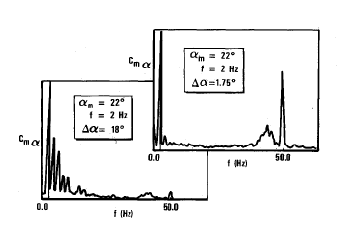
\includegraphics[scale=1.5]{Cm_PSD_Boer1}
\caption{Power spectrum plots showing harmonics in responses due to inputs of different amplitudes \cite{Boer2}.}
\label{fig:Cm_PSD_boer}
\end{figure}
%\end{wrapfigure}

The nonlinear nature of the variation of aerodynamic loads due to large amplitude inputs is evident from their power spectrum maps. As seen in Fig.(\ref{fig:Cm_PSD_boer}), second and third order harmonics of the input frequency are excited to a significant level for input amplitude of $18^o$, while these are absent for amplitude of $2^o$. These harmonics are also observed for pressure measurements at a particular location on a double-delta wing \cite{Boer2}. 

The nonlinear nature of unsteady variations can be attributed to changing value of the time-scale parameter over the range of angle-of-attack under consideration; and different time-scales of pressure variation on the wing for pitching motion. When the external pressure gradient on the wing was varied (??) the time-constant for change in vortex breakdown location was found to be different. This implies that the time-constant for pitch-up motion is greater than the time-constant for pitch down motion. For sinusoidal variation in angle-of-attack, the changing time-constant with the phase of oscillation causes a non-elliptic variation in aerodynamic loads which shows that the unsteady variation is nonlinear.

% a. Memory effect causing unsteady dependence b.	Amplitude/Frequency dependence c.	 Super-harmonics in loads and pressure d.	Time-scale in pitch-up and pitch-down e.	Static hysteresis, Critical states crossing

\section{PDEM and VVM modeling approaches}

% While a simple first order transfer function can model the mildly nonlinear variations in normal force coefficient, a nonlinear model structure is essential for accurately modeling the pitching moment coefficient. This is illustrated in the next section. In this section, properties of the both these model structure that make them useful for modeling nonlinear unsteady aerodynamic coefficients are presented.

Formulation of the two model structures PDEM and VVM are presented in this section to highlight the mathematical formalism and features of these two structures which make them useful for identification of a variety of unsteady aerodynamic systems. The unique advantage of using both these model structures for modeling the unsteady loads on a delta-wing aircraft is that these capture linear unsteady variation for small amplitude change in angle-of-attack and nonlinear variation due to large amplitude change in angle-of-attack seamlessly. A parameter estimation methodology for use with forced oscillation wind tunnel test data is presented and it is suitable to both of the model structures.  A comparison of the results obtained from these approaches is presented in the next section.

The PDEM and VVM models are formulated as incremental components of load due to unsteady aerodynamics over the quasi-steady variation included in the aero-database of the aircraft. These models can be applied to the coefficients $C_Z, C_m$ and are collectively represented by $C_a$ in the following derivations. Similar derivation applies to $C_l, C_n$, and the resulting structure are presented at the end of this section. The incremental component captures the dependence of load on history of aircraft dynamic states. Both PDEM and VVM are in the form of differential equations, based on the theory of dynamic systems represented in State-space form and Volterra Series respectively. 
\begin{eqnarray}
\label{eq:Czt}
C_a(t) = C_{a,st}(\alpha (t))+ C_{a_q}(\alpha (t))\frac{q(t) \bar{c}}{2V} + C_{dyn}(\alpha (t), \dot{\alpha}(t))
\end{eqnarray}
An aerodynamic load represented by $C_a(t)$ can be split into the components of steady and unsteady variations, as a function of $\alpha,\dot{\alpha}$ and $q(t)$, as given in Eq.(\ref{eq:Czt}). $C_{a,st}(\alpha)$ is the steady state value at each angle-of-attack, and it is known from static wind tunnel tests. $C_{a_q}$ represents the incremental effect of steady pitching motion on $C_Z, C_m$. This component is usually small and cannot be inferred directly from wind tunnel test data. It is estimated during the process of parameter estimation. Some computational methods for the case of symmetric airfoils have been proposed recently [khrabrov-greenwell]. $C_{dyn}(t)$ represents the unsteady component of load determined by rate of change in angle-of-attack, assuming that the side-slip angle is held constant.

The component $C_{dyn}(t)$ is identified from dynamic wind tunnel test data. Any change in angle-of-attack produces a non-zero value of $C_{dyn}(t)$, and it converges to zero with a certain time-lag when angle-of-attack is held steady. Hence, $\dot{\alpha}(t)$ is the input to the mathematical equations governing $C_{dyn}(t)$. This  has a stable equilibrium at $C_{dyn}(t)=0,\dot{\alpha}(t)=0$ over the domain $\alpha \in [-90^o,90^o)$. Also, the time-constant for unsteady change in $C_{dyn}(t)$ is the same as that for $C_a(t)$. Hence, PDEM and VVM contain a mathematical formulation for $C_{dyn}(t)$ which is sufficient to capture the nonlinear unsteady variation of aerodynamic loads.

necessary and sufficiency conditions for component splitting of the loads.??

\subsection{Polynomial-nonlinearity Differential Equation Structure}
Systems for which current state depends on the history of inputs, also called systems-with-memory, can be modeled by a generic nonlinear differential equation of the type as in Eq.(\ref{PoDE}). Assume that this system is single-input-single-ouput, analytic and input-affine. (cite Van der Scahft, and implications of this structure from systems theory??)
\begin{eqnarray}
\label{PoDE}
\frac{d}{dt}x(t) + \sum_{i=2}^{n} a_{i} x(t)^{i} = \sum_{i=1}^{n} b_{i} x(t)^{i-1}u(t); \, \, t\geq0 \\ \nonumber
y(t)= C x(t)+y_0(t); \, \, x(0)=0
\end{eqnarray}
where, $x(t)$ and $u(t)$ are the state and input terms respectively, while $\{(a_i,b_i) \, \forall \, i \in [1 \, n]\}$ are constant scalars. Since, the output $y(t)$ is simply a scalar multiple of the state, we consider only the input-state dynamics in further derivations. PDEM is formulated based on this equation as follows.
 \begin{eqnarray}
\label{eq:Abramov-Goman2}
\Delta C_a(\alpha) &=& C_{a,st}(\alpha) - C_{a,att}(\alpha) \nonumber \\
\frac{d C_{dyn}}{dt} + \frac{1}{\tau} C_{dyn} &=& k_1 \Delta C(\alpha) \dot{\alpha} +  \sum_{j=2}^{j=m} k_i (\Delta C(\alpha) - C_{dyn})^m
\end{eqnarray} 
In this equation, $C_{a,att}$ is a theoretical aerodynamic load that would exist assuming there is no vortex breakdown on the wings at stall and post-stall angle-of-attack range. It can be obtained using, for example, Polhamus suction analogy. $m$ is the degree of polynomial terms of $(\Delta C(\alpha) - C_{dyn})$. Since, $\Delta C(\alpha) \, vs. \, \alpha$ is approximately linear, any degree of this term can only produce a first harmonic to sinusoidal inputs. Thus the nonlinear nature of unsteady variation of loads is captured by the polynomial terms in $C_{dyn}(t)$.

The value of $m$ is chosen based on extent of data, nonlinear nature of variations and accuracy of the model desired. 
For $m=1$ in Eq.(\ref{eq:Abramov-Goman2}), it becomes a simple linear first order transfer function. Since $\Delta C(\alpha)$ is a function of $\alpha$, it can account for mild nonlinearities associated with large amplitude change in angle-of-attack. Thus, if the variation of coefficient is mildly nonlinear, $m=1$ is sufficient. A maximum of $m=3$ is required to model the nonlinear nature in several case studies undertaken by the authors. $k_i$ are the parameters of the model and are identified using forced oscillation test data as presented later in this section.

A characteristic of PDEM is its capability to capture static hysteresis concurrently with unsteady variation observed for loads like $C_Z$, $C_m$ and $C_l$ for some wings and airfoils. This is true for $m=3$ and setting a constraint on solutions of Eq.(\ref{eq:Abramov-Goman2}) to have two real and one imaginary roots. The real solutions correspond to the two branches of the static hysteresis curve while the imaginary solution acts like a seperatix between the two real ones, as shown in Figure (). However, the aerodynamic loads on a Delta-wing aircraft do not exhibit any static hysteresis at low-Mach number. Hence, a constraint is set on the solutions to have one real and an imaginary pair of roots.

This model has been satisfactorily used to model the nonlinear unsteady variation of delta-wing aircraft like GTA, F16XL and Delta-65. 

\subsection{Volterra Variational Model Structure}
Volterra series is a functional expansion of the response of a nonlinear dynamical system with memory to any arbitrary input, proposed by Vito Volterra in 1924 \cite{Volterra}. It was first used for modeling nonlinear electrical systems by N. Weiner in 1952, and since then it has been successfully used for modeling many Bio-medical and Electrical systems \cite{Marmerelis}. It's application to modeling aerodynamic loads has been attempted using approximation of the integral formulation by P. Reisenthel and W.Silva \cite{ReiKernel,SilvaUnst}. The accuracy of their results and the interpretation of their approximation have been unsatisfactory.
\begin{eqnarray}\label{Voltseries}
x(t)&=&h_0(t) + \int_{0}^{\infty} h_1(\tau_1)u(t-\tau_1)d\tau_1 + \sum_{n=2}^\infty \int_{0}^{\infty} \cdots \int_{0}^{\infty}{h_n(\tau_1,\cdots,\tau_n)\prod_1^n u(t-\tau_n)d\tau_n}
\end{eqnarray}

Volterra series consists of linear sum of the convolution of the polynomial terms of input and higher dimensional functionals called the kernels, as given in Eq.(\ref{Voltseries}). This is Volterra series for a Single-input-single-output system. The integrand $h_n(\tau_1,...,\tau_n)$ is called $n$-th symmetric kernel of Volterra series. The kernels are unique functionals characterising the system dynamics. For a linear system, only the first kernel $h_1(\tau_1)$ is significant, and all higher order kernels are zero. Volterra series is a direct superposition of the responses of kernels to a given input. The infinite series is truncated to first few terms for modeling physical systems and this has been shown to converge to a single stable steady-state solution for certain bounded inputs\cite{BoydChua}. 

Direct estimation of Volterra kernels requires special experimental data from wide-band inputs with large number of harmonics [ref]. Since such experiments are infeasible to be conducted in a wind tunnel or an aircraft in flight, the methods presented in literature are based on approximation of kernel shapes. In the derivation presented here, the kernel shapes are constrained by parameters of the PDEM model, to get a parametric form of the Volterra series called the Volterra variational equations.

The Volterra variational equations can be obtained as the Volterra series representation of the system in Eq.(\ref{PoDE}) \cite{Rugh}. Let the term for response of kernel $h_n(\cdot)$ be represented by so-called kernel-state $x_n(t)$. Then Eq.(\ref{Voltseries}) becomes,
\begin{eqnarray}
x(t) = x_1(t)+x_2(t)+x_3(t)+...+x_n(t)+...
\end{eqnarray}
Considering this form of the Volterra series, Volterra variational equations can be derived in time-domain as given in \cite{Rugh}, and in frequency domain as given in [Thesis].
\begin{eqnarray}
\label{eq:VVM_1}&&\frac{d}{dt}x_1(t) +a_1 x_1(t)= b_1 u(t)\\
\label{eq:VVM_2}&&\frac{d}{dt}x_2(t)+a_1 x_2(t)+ a_2x_1^{2}(t)= b_2 x_1(t) u(t)\\
\label{eq:VVM_3} &&\frac{d}{dt}x_3(t)+a_1 x_3(t)+ 2 a_2x_1(t)x_2(t)+ a_3 x_1(t)^{3}= b_2 x_2(t)u(t)+ b_3 x_1(t)^2 u(t)\\ \nonumber
&...
\end{eqnarray}
where, $x_1(0)=0$, $x_2(0)=0$, $x_3(0)=0$. $a_1=\frac{1}{\tau}$ is the time-constant of system dynamics. This is an infinite series, but just like Volterra series it can be truncated to first few terms for practical applications. These equations are parametric and differential, which makes them suitable for estimation using variety of wind tunnel test data. 

Volterra-variational-model of unsteady aerodynamic loads can be formulated from Volterra variational equations as follows. From Eq.(\ref{eq:Czt}), it is evident that $C_a(t)$ converges to $C_{a,st}(t)$  with a finite time delay when $\dot{\alpha}=0$, and its time-scale is the same as that governing $C_{dyn}(t)$. For a time-invariant system all the parameters of the model can be considered to be constants. In case of unsteady aerodynamics, the variation in loads depends on initial angle-of-attack, and its characteristic time-scale is a function of angle-of-attack. This angle-of-attack dependence is accounted for by considering the model parameters as function of angle-of-attack. Any constant value of the parameters can reproduce amplitude and frequency dependence of loads as observed in forced oscillation wind tunnel test data. Therefore, all the parameters are considered to be functions of instantaneous $\alpha$. Thus, the model for $C_{dyn}(t)$ becomes as in Eq.(\ref{eq:UAM}).
\begin{eqnarray}
\label{eq:UAM}
%C_Z(\alpha,t) &=& C_{Z_{st}}(\alpha) + C_{dyn}(t) \nonumber\\
C_{dyn}(t)&=& x_1(t) + x_2(t) +x_3(t) \nonumber \\
\dot{x}_1(t)&=&a(\alpha)x_1(t)+ K_1(\alpha)\dot{\alpha}(t), \, \, x_1(0)=0 \nonumber \\
\dot{x}_2(t)&=&a(\alpha)x_2(t)+ K_{21}(\alpha)x_1^{2}(t) + K_{22}(\alpha)x_1(t)\dot{\alpha}(t), \, \, x_2(0)=0 \nonumber \\
\dot{x}_3(t)&=&a(\alpha)x_3(t)+ K_{21}(\alpha)x_1^{3}+ K_{31}(\alpha)x_1(t)x_2(t)  + \nonumber \\
&& K_{32}(\alpha)x_2(t)\dot{\alpha}(t) + K_{22}(\alpha)x_1^{2}(t)\dot{\alpha}(t) , \, \, x_3(0)=0
\end{eqnarray}
In these equations, different notations for the parameters of VVM are used in order to avoid confusion between the equivalence of PDEM and Volterra variational equations. The parameters have been redefined as, $a_1= a $, $b_1=K_1$, $a_2=K_{21}$, $b_2=K_{22}$, $a_3=K_{31}$, $b_3=K_{32}$.

The VVM contains differential equations for second and third kernels containing nonlinear terms in $x_1, x_2, x_3$. The parameter values in these equations give a certain definite kernel shape, and this has been obtained computationally in \cite{OmranACC}. It is important to note that, in this formulation there is no assumption regarding the type of data implicitly or explicitly, as done in other model structures proposed in literature. Therefore, this model structure is generic and can be further extended to any application, and estimated from any data using an appropriate approach. The parameter functions are estimated from small and large amplitude forced oscillation wind tunnel test data, as presented in the next section.

\subsection{Parameter Estimation Approach}
The model parameters are estimated by two-step regression method presented in this section using forced oscillation wind tunnel test data. This method can be applied to both PDEM and VVM structures. This is because both the model structures can be approximated to a simple first order differential equation considering small amplitude input. The difference is in their nonlinear dynamic features.

In a forced oscillation wind tunnel test, a scaled model of the aircraft is mounted on a special rig capable of moving it such that change in $\alpha$ is sinusoidal while $\beta$ remains constant at a certain value. This test is typically performed for $3-5$ frequencies about a certain mean angle-of-attack in the stall region for a wide range of amplitudes. The tests which use an amplitude of $3^o-5^o$ are called small amplitude tests while large amplitude tests use amplitudes in the range of $10^o-30^o$.  In the two step-regression method, first the data is classified into small and large amplitude test data. While small-amplitude test data is used for estimating the first-order or reduced-order linearised forms of the model structures, large-amplitude test data is used to refine the responses to capture the nonlinear nature of unsteady variations.

In the first step, the linearized form of the models for a small amplitude sinusoidal change in angle-of-attack is shown to provide a linear relationship between in-phase and out-of-phase derivatives. Therefore, the in-phase and out-of-phase derivatives from at least three different frequencies, are used to estimate the model parameters ($\tau, K_1$) of VVM or ($\tau, k_1$) of PDEM by linear regression. The remaining parameters that introduce nonlinear corrections are estimated by output-error method using the entire set of large amplitude forced oscillation data.

In a small amplitude forced oscillation test, the wind tunnel model is oscillated in pitch in a sinusoidal motion as $\alpha(t)= \alpha_0 + \Delta \alpha sin(\omega t)$. The measured normal force or pitching moment coefficient $C_a(t)$ is converted to in-phase derivative $C_{a_{\alpha,\omega_0}}(\alpha_0)$ and out-of-phase derivative $C_{a_{\dot{\alpha},\omega_0}}(\alpha_0)$ by harmonic analysis of the time-series data. The pitching frequency is non-dimensionalised as $ \bar{\omega}=\frac{\omega \bar{c}}{2 V}$, where, $\bar{c}$ is mean aerodynamic chord and $V$ is the air speed. Therefore, the steady-state response of the normal force coefficient measured in a wind tunnel test is given by,
\begin{eqnarray}
\label{Cztsmall}
C_Z(t) = C_{Z_0}(\alpha_0) + C_{Z_{\alpha,\omega_0}}(\alpha_0) \Delta \alpha \sin(\omega t) + C_{Z_{\dot{\alpha}},\omega_0}(\alpha_0) \bar{\omega}  \Delta \alpha \cos(\omega t)
\end{eqnarray}

Now consider the response of VVM in Eq.(\ref{eq:UAM}) to sinusoidal pitching input. For small amplitude input, the model response is expected to be approximately linear. Hence, only the first kernel state is significant, which implies $C_{dyn}(t)=x_1(t)$. Thus, the output $C_{dyn}(t)$ to the input $\dot{\alpha}= \Delta\alpha \bar{\omega} \cos(\omega t)$ is given by,
\begin{eqnarray}
\dot{C}_{dyn}(t) &=& \dot{x}_1(t) \nonumber \\
&=& a(\alpha_0)x_1 + K_1(\alpha_0) \dot{\alpha}(t) \nonumber \\
&=& a(\alpha_0)x_1 + K_1(\alpha_0) \bar{\omega}\Delta\alpha \cos(\omega t)
\end{eqnarray}
Solving this differential equation, the steady-state solution $C_{dyn}(t)_{ss}$ is obtained as,
\begin{eqnarray}
C_{dyn}(t)_{ss} &=& \frac{K_1 \Delta \alpha \bar{\omega}^2 }{a^2 + \bar{\omega}^2} sin(\omega t)  -  \frac{K_1 \Delta \alpha \bar{\omega} a }{a^2 + \bar{\omega}^2} \cos(\omega t)
\end{eqnarray}
Then, Eq.(\ref{eq:Czt}) is linearized at $\alpha_0$ and substituting the above equation in it gives the total normal force coefficient as,
\begin{eqnarray}
\label{eq:modelresp}
C_a(t)_{ss} &=& C_{a_0}(\alpha_0) + C_{a_{\alpha,st}}(\alpha_0) \Delta \alpha sin(\omega t) +  C_{a_q}(\alpha_0) \bar{\omega} \Delta\alpha \cos(\omega t) \nonumber \\
&+& \frac{K_1 \bar{\omega}^2 }{a^2 + \bar{\omega}^2} \Delta \alpha sin(\omega t)  -  \frac{K_1 a }{a^2 + \bar{\omega}^2} \Delta \alpha  \cos(\omega t)
\end{eqnarray}

Equations (\ref{Cztsmall}) and (\ref{eq:modelresp}) represent steady state variation of the aerodynamic coefficient from the wind tunnel test and VVM respectively. Hence, comparing them gives the relation between model parameters and experimental derivatives as,
\begin{eqnarray}
\label{eq:2step}
C_{a_{\alpha,\omega_0}}(\alpha_0) &=&  C_{a_{\alpha,st}}(\alpha_0) +  \frac{K_1 \bar{\omega}^2 }{a^2 + \bar{\omega}^2}  \nonumber \\
C_{a_{\dot{\alpha},\omega_0}}(\alpha_0) &=&  C_{a_q}(\alpha_0)  -  \frac{K_1 a }{a^2 + \bar{\omega}^2}
\end{eqnarray}
Rearranging the terms in Eq.(\ref{eq:2step}), a linear relation between $C_{a_{\alpha,\omega_0}}(\alpha_0)$ and $C_{a_{\dot{\alpha},\omega_0}}(\alpha_0)$ is evident in Eq.(\ref{eq:linregress}). 
\begin{eqnarray}
\label{eq:linregress}
C_{a_{\alpha,\omega_0}}(\alpha_0) &=& a C_{a_{\dot{\alpha},\omega_0}}(\alpha_0) + [ C_{a_{\alpha,st}}(\alpha_0) + K_1 - C_{a_{q}}(\alpha_0) ]
\end{eqnarray}

The values $C_{a_{\alpha,\omega_0}}(\alpha_0)$ and $C_{a_{\dot{\alpha},\omega_0}}(\alpha_0)$ are known for at least three frequencies from SAFO test data at each $\alpha_0 \in [25^o \, 90^o]$ . Hence, using Eq.(\ref{eq:linregress}), $a(\alpha_0),K_1(\alpha_0)$ at each $\alpha_0$ in the stall region can be estimated by linear regression method, further detailed in APPENDIX $1$.

However, it is important to consider noise and nonlinear nature of data before it is used in parameter estimation. The forced oscillation tests can be complicated due to sting vibration; external disturbances affecting the flow; excitation caused by vortex shedding etc. Due to estimation of in-phase and out-of-phase derivatives from SAFO data, noise is filtered to some extent. It is important to check the presence of any higher order harmonics in the load response data to ensure that the variation is actually linear. This is especially true when $\Delta \alpha >3^o$.

\subsection{Estimation of Nonlinear Model Parameters using LAFO Data}
The values of parameters $a(\alpha_0),K_1(\alpha_0)$ are estimated at certain angle-of-attack intervals, typically $5^o$. However, the time-constant of vortex dynamics changes significantly over that interval of angle-of-attack. Hence, the parameters are defined as functions of angle-of-attack, with their value defined by linear interpolation over the interval. This makes the unsteady aerodynamic model nonlinear for very large-amplitude changes in angle-of-attack. 

It is important that the resulting nonlinear response of the model to be identified should be consistent with the nonlinear variations captured in the LAFO data. The values of estimated parameters in the first step may have significant $2 \sigma$ confidence bounds at some $\alpha_0$. Hence, defining a parameter function by simply using the linear interpolation of the values from the first step is inadequate. Therefore, the LAFO data is first used to tune the parameter functions $(a(\alpha),K_1(\alpha))$. This is done by considering the parameter value at each $\alpha_0$ as a free node with confidence bounds are constraints. Then the estimated parameter functions $(a(\alpha),K_1(\alpha))$ are frozen, and higher order kernel states are included in the model structure. 

For large amplitude sinusoidal inputs, the nonlinear nature of variations is indicated by the presence of higher order harmonics. In case of VVM, the harmonics in the response are well defined by each kernel state. It is know that, $x_1$ produces only first harmonic; $x_2$ produces only second harmonic, $x_3$ produces first and third harmonic  components in the response. Therefore, number of kernel states required in the nonlinear model to get satisfactory results can be determined by scanning the power-spectrum-density maps of the entire data set. Since VVM actually contains parameter functions and not just scalars, this is a sufficiency condition. In other words, if the PSD of LAFO data contains a maximum of second harmonic, including $x_2$ in the model structure is sufficient.

The parameters of higher order kernel states are estimated by output-error method. Since VVM is linear in parameters, the estimates obtained from output-error method are also the maximum likelihood estimates \cite{Morelli}. The parameter functions of higher order kernel states are defined by considering a number of nodes in the stall-region and linear interpolation between them. As known from the system identification theory, a larger number of node-points than essential causes the variance and bounds of the estimated values to be larger. Thus,  although larger number of node-points improve the accuracy of results, it reduces the fidelity of the model for simulation using random inputs.

A proper choice of optimization algorithms is important because the parameters need to be estimated using a large data set. The total root-mean-square-error between model output and experimental response across the entire data set is used as the cost function. A combination of both gradient and steepest-descent based methods are used in the current study. All the concepts presented here are illustrated in the case studies presented in the next section.

\subsection{Phenomenological interpretations of VVM}
Linearised form of VVM and interpretation of its time-scale parameter. Effect of nonlinear terms on time-scale parameter etc..


The time-scale of unsteady variation depends on energy of input, which in forced oscillation tests is represented by amplitude of input. The effective time-constant of response of an unsteady load is different for small and large amplitude harmonic input. This phenomena is inherent to VVM and holds true for PDEM under certain conditions. This can be explained considering a mildly nonlinear coefficient which is adequately modeled by the two-state VVM in Eq.(\ref{eq:UAM2term1}). An important property of Volterra series and hence VVM, is that the first kernel ($x_1(t)$) produces the most dominant contribution to response, that is $\| x_1\| > \| x_2\|$. Hence, it can assumed that $C_{dyn} = x_1$ in Eq.(\ref{eq:UAM2term2}) and then the differential equation for $C_{dyn}(t)$ can be approximated as,
\begin{eqnarray}
\label{eq:UAM2term1}\dot{C}_{dyn}(t)&=& \dot{x_1}(t) + \dot{x_2}(t)  \\
            &=&a(\alpha)x_1(t)+ K_1(\alpha)\dot{\alpha}(t) + a(\alpha)x_2(t)+ K_{21}(\alpha)x_1(t)\dot{\alpha}(t) + K_{22}(\alpha)x_1(t)^2 \nonumber \\
\label{eq:UAM2term2}            
&\simeq& [a(\alpha) + K_{21}(\alpha) \dot{\alpha}(t) ]C_{dyn}(t) + K_{22}(\alpha) C_{dyn}(t)^2 + K_1(\alpha)\dot{\alpha}(t)
\end{eqnarray}
where $\alpha(t)$ is replaced by $\alpha$. 

%In this representation, the effective time-constant for unsteady variation of $C_{dyn}(t)$ is the effective time-constant of nonlinear unsteady variation of the aerodynamic coefficient, which is due to large amplitude pitching motion input.

Equation (\ref{eq:UAM2term2}) is nonlinear in $C_{dyn}(t)$, and excluding the input term the remaining expression has two solutions, $C_{dyn,1}=0$ and $C_{dyn,2}=\frac{-a(\alpha)}{K_{22}(\alpha)}$.  The solution $C_{dyn,2}$ is unrealistic for typical values of $a(\alpha), K_{22}(\alpha)$ presented in the next section. So $C_{dyn,1}=0$ is the only realistic solution. The effective time-constant for equilibrium at $C_{dyn,1}=0$ is given by $[a(\alpha)+K_{21}(\alpha)\dot{\alpha}]$. In this expression, the effective time-constant depends on $\dot{\alpha}$, which implies that it is determined by the direction of pitching motion. For a stable VVM, $a(\alpha)<0$, and the estimated values of $K_{21}(\alpha) \leq 0$ as seen in the next section. Therefore, in pitch-up motion, $[a(\alpha)+K_{21}(\alpha)\dot{\alpha}]$ has a larger magnitude than in pitch-down motion. This has been observed to be true for unsteady variation of normal force or pressure variation in at least two experimental studies discussed in the following paragraphs.

Reisenthel.et.al observed in their experiments on the effect of oscillating fin on vortex breakdown location that the time-constant for upstream motion of vortex breakdown location is larger than that for downstream motion \cite{ReiFin}. Upstream motion of vortex breakdown location corresponds to pitch-up and downstream motion to pitch-down. Therefore, the time-constant for pitch-up is larger than that in pitch-down motion.

In dynamic wind tunnel test studies reported in \cite{AGARDAR305} for pitch-up and pitch-down motion inputs, the values of time-constant were estimated separately for the two input cases. It was observed that the time-constant in pitch-up motion is greater than in pitch-down motion in the stall region. This phenomena has also been observed consistently for some other experimental studies report in the review paper \cite{Gursul}. Thus, the fundamental effects of different effective time-constants for small amplitude, large amplitude pitch-up and large amplitude pitch-down motion inputs are incorporated inherently in VVM as evident from Eq.(\ref{eq:UAM2term2}).

The linearized equations of VVM in Eq.(\ref{eq:linregress}) are similar to that obtained by Abramov.et.al \cite{Abramov1}. A comparison of the two models gives $K_1(\alpha)=\Delta C_Z(\alpha)= C_{Z_{att}}(\alpha)- C_{Z_{st}}(\alpha)$. Here, $C_{Z_{att}}(\alpha)$ is the normal force with no flow separation or vortex breakdown on the wings, that can be obtained from the Polhamus Suction-analogy method. Therefore, the dynamic gain parameter function $K_1(\alpha)$ in the VVM actually represents the loss in normal force due to vortex breakdown on the wings.

%The effect of the nonlinear terms in the differential equation $\dot{x_2}(t)$ in VVM on the model response has been recently presented in \cite{OmranACC}. In response to harmonic inputs, the nonlinear terms in this differential equation effect the steady state and initial response characteristics. It is noted that the bilinear term $K_{22}(\alpha)x_1 u$ does not modify the effective time-constant and therefore the transient response, but it changes the steady state oscillation cycle. The quadratic term $K_{21} x_1^2$ changes the settling time or the effective time-constant of the response. This shows that inclusion of just the second kernel state can reproduce the nonlinear phenomena in unsteady variation of coefficients. Thus, the parameters of these terms tune the effective time-constant of VVM to be dependent on the amplitude and rate of pitching motion input.

\section{Identification Case Studies}
In this section, identification of the unsteady models of $C_Z$ and $C_m$ of GTA for VVM and PDEM are presented. Identification of the linear form of both the models using SAFO data is common, while the estimation of nonlinear models is done separately using LAFO data. In the end, results from VVM and PDEM models are compared for accuracy.

\subsection{Data for GTA}
\begin{figure}[t]
\centering
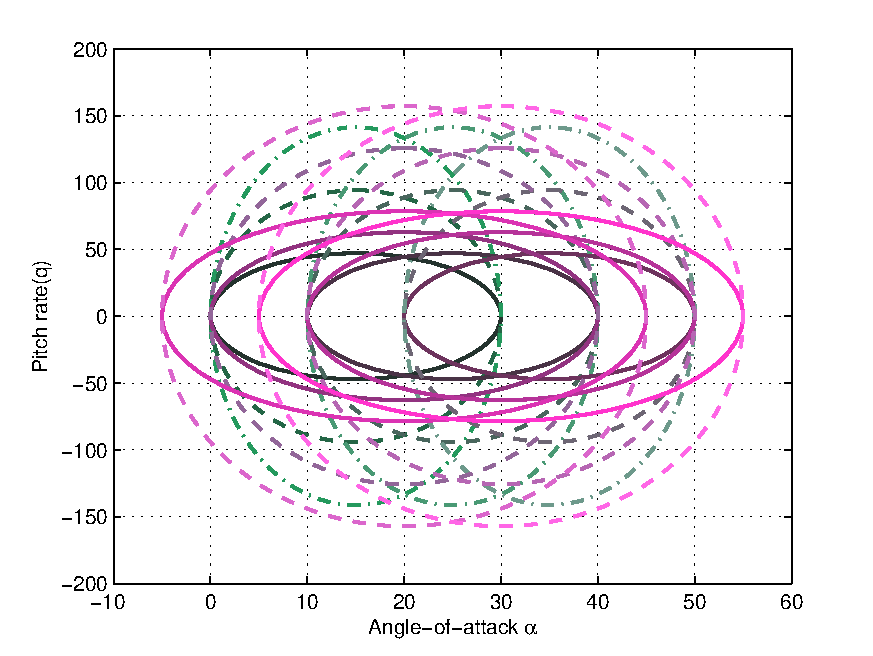
\includegraphics[scale=0.8]{GTA_inputs}
\caption{Range of inputs used in LAFO tests of GTA; solid-line $f=0.5Hz$, dash-line $f=1Hz$, dash-dot-line $f=1.5Hz$.}
\label{fig:GTA_inputs}
\end{figure}
GTA is a delta-wing configuration research aircraft with leading-edge sweep angle of $60^o$. It has a typical geometry of high-performance, high-maneuverability aircraft. The wind tunnel tests were conducted on a $1:15$ scale model of GTA in an industrial grade wind tunnel. Static and forced oscillation wind tunnel test data are partially available for the current research.

Small amplitude forced oscillation tests were conducted with inputs of amplitude $3^o$ at three frequencies $(0.5,1,1.5) Hz$. These tests were performed at angle-of-attack intervals of $5^o$ in $[0^o \, 90^o]$  range. The sensors recorded variations in normal force and pitching moment coefficients at a frequency of $100 Hz$. These response data are reduced to in-phase and out-of-phase derivatives by numerical computation of Fourier coefficients at respective input frequencies. 

%Only these derivatives are available for modeling. The $2\sigma$ confidence bounds of the estimated values of these derivatives are not available.

Large amplitude forced oscillation data set is comprehensive. Angle-of-attack inputs of amplitudes of $15, 20$ and $25$ degrees, at mean angles-of-attack of $[15, 25, 30, 35, 45] \deg$ and frequencies of $[0.5,1,1.5] Hz$  were used in these tests. This data-set covers wide range of pitch-rate, frequency and amplitude combinations as visualized in Fig.(\ref{fig:GTA_inputs}). The corresponding non-dimensional frequencies of pitch oscillation are $[0.0024 \, 0.0047 \, 0.0071]$. It is comprehensive enough to capture the effects of  nonlinear unsteady aerodynamics relevant to aircraft's operational bandwidth.

%A limited set of raw wind tunnel data from large amplitude forced oscillation tests is also available, but only for $C_Z$. 
Static wind tunnel test data from the same rig and using the same model for all the force and moment coefficients were recorded at angle-of-attack intervals of $5$ degrees. The overall quality of the data can be considered to be on par with the best available in literature.

%---------------Identification of Cz and Cm of GTA--------------------------------------------
\subsection{Identification of Normal force coefficient of GTA}
%The parameters $(a(\alpha_0),K_1(\alpha_0))$ of the first-kernel state are estimated using SAFO data. Then, the LAFO data is used to tune the model's nonlinearity properties by tuning the parameter functions $(a(\alpha),K_1(\alpha))$.

%\subsection{Estimation using SAFO data}

%Figures and results to be discussed:
%\begin{enumerate}
%\item Linear relation between in-phase and out-of-phase derivatives of CZ
%\item Estimated parameters from SAFO data, with bounds of Cz, Cm
%\item Simulation results for VVM1 of CZ with raw data
%\item Power spectrum density of LAFO for CZ and CM
%\item Simulation results for VVM1 + VVM3 + PDEM3 of Cm
%\end{enumerate}

\begin{figure}
\centering
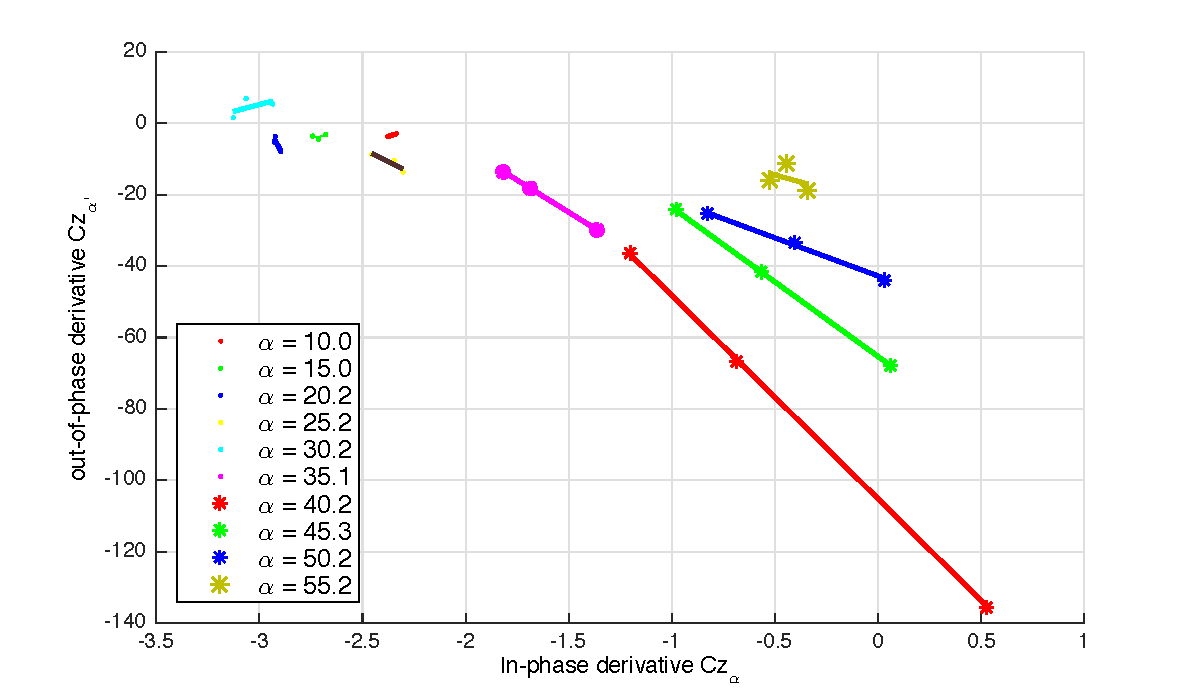
\includegraphics[width=100mm]{CZ_ip_op}
\caption{Linear relation between In-phase vs. Out-of-phase derivatives for $C_Z$ of GTA, from SAFO data.}
\label{fig:GTA_Cz_Ts}
\end{figure}
For $C_Z$ of GTA, as seen in Fig.(\ref{fig:GTA_Cz_Ts}), the linear relationship between in-phase and out-of-phase derivatives holds good. The separation between the points for different frequencies is distinct only in the range $\alpha \in (30^o \, 55^o)$. This is also the region of dominant unsteady aerodynamics of the aircraft. Hence, $a(\alpha_0),K_1(\alpha_0)$ are estimated in this angle-of-attack range.

Linear regression is performed by iterative Weighted-Least-Squares method [ref]. The estimation error covariance matrix is computed in each iteration, and its inverse is used as weighting matrix for the next iteration. The final step is defined by negligible change in error covariance matrix. It is then is used to compute the confidence bounds on estimated values of parameters $(a(\alpha_0),K_1(\alpha_0))$.

\begin{figure}
\centering
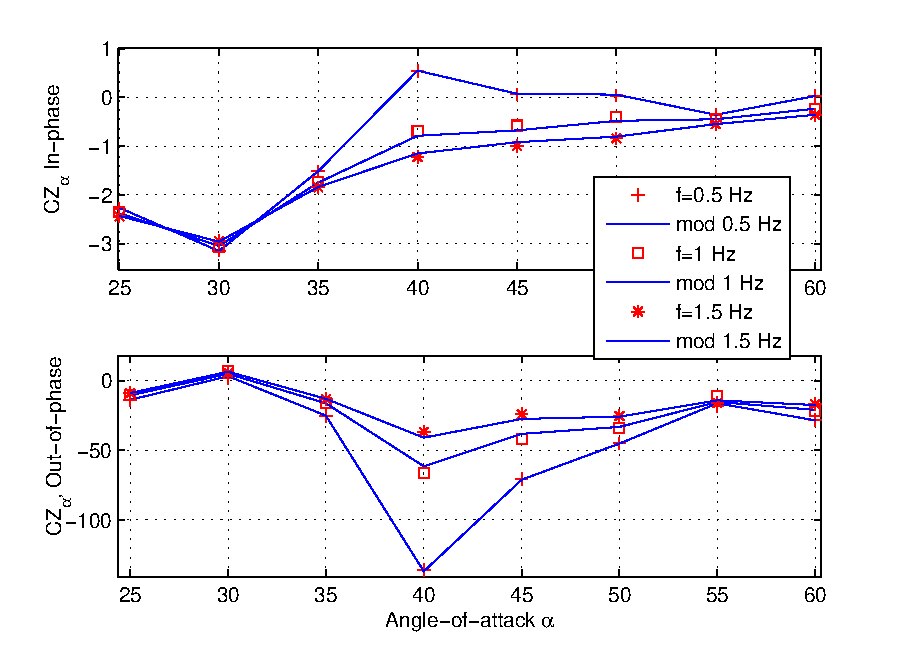
\includegraphics[width=100mm]{GTA_Cz_SA}
\caption{Comparison of in-phase and out-of-phase derivatives from the estimated model and experimental data for $C_Z$ of GTA.}
\label{fig:GTA_Cz_res}
\end{figure}
\begin{figure}
\centering
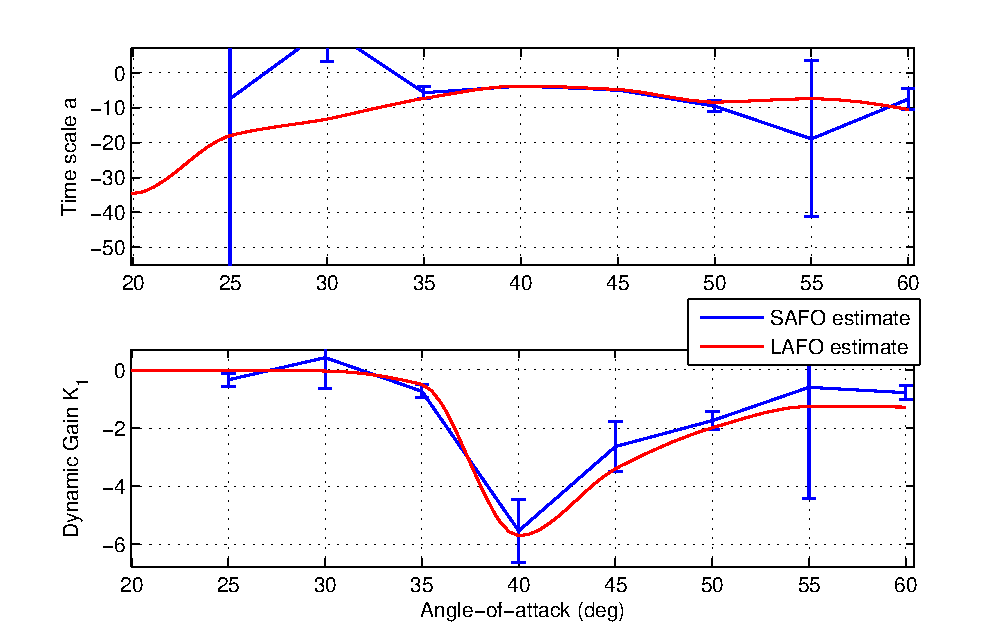
\includegraphics[width=100mm]{GTA_Cz_Par}
\caption{Estimated bounds on the first kernel-state parameters and parameter functions for $C_Z$ of GTA.}
\label{fig:GTA_Cz_Par}
\end{figure}

The steady state solutions of the model are required to match static test data. The derivative of $C_Z \, vs. \, \alpha$ curve, denoted as $C_{Z_\alpha,st}(\alpha_0)$, are estimated from static wind tunnel data, and used as a constraint equation in the second step of regression. Since the static data for $C_Z$ of GTA is available at only $5 \deg$ intervals of angle-of-attack, its derivative has a high uncertainty. This becomes an important issue in the stall angle-of-attack region where $C_{Z,st}(\alpha)$ changes rapidly. Hence, $C_{Z,st}(\alpha)$ is curve-fitted with a $7$-th degree polynomial function and then differentiated to get $C_{Z_\alpha,st}(\alpha_0)$. 

%Also, the oscillation in angle-of-attack is over a small range of $\alpha=6^o$. Hence, the approximation of the value of slope by curve-fitting is likely to be close to the actual value.

%Since the co-variances of in-phase and out-of-phase derivatives were not available


The experimental data and model prediction using the estimated values of parameters are found to match accurately as seen in Fig.(\ref{fig:GTA_Cz_res}). The goodness-of-fit for the estimated values is given by parameter variance or $95\%$ confidence bounds on estimated values at each $\alpha_0$. The parameter bounds are indicated by vertical bars in Fig.(\ref{fig:GTA_Cz_Par}), which show that the estimates are acceptable for $\alpha \epsilon [35^o \, \, 50^o]$. 

Unsteady aerodynamics is not sufficiently excited by the small amplitude inputs outside $\alpha \epsilon [35^o \, \, 50^o]$. Hence, signal-to-noise ratio is poor, and linear relation between in-phase and out-phase derivatives is unclear, as seen in Fig.(\ref{fig:GTA_Cz_Ts}). Thus, SAFO data indicates unsteady nature of load only for $\alpha \in [30^o \, 55^o]$, while At $\alpha=(25^o,60^o)$ that SAFO data is unreliable. But LAFO data indicates that unsteady component of loads is significant for $\alpha \in [25^o \, 60^o]$. Hence, $(a,K_1)$ are estimated over the range $\alpha=[25^o , 60^o]$ using LAFO data in the next step.

Outside the stall angle-of-attack region, i.e. $\alpha \in \{[0 \, 25^o] ,[60^o \, 90^o]\}$, $C_{dyn}(t)$ is expected to be zero. This is affected by considering the magnitude of time-scale parameter to be relatively very large of about $a<-20$; while $K_1$ is made zero, as seen in Fig.(\ref{fig:GTA_Cz_Ts}). The linear unsteady effects in this region are represented by the damping derivative (out-of-phase derivative) term included in the aero-database.

\begin{figure}
\centering
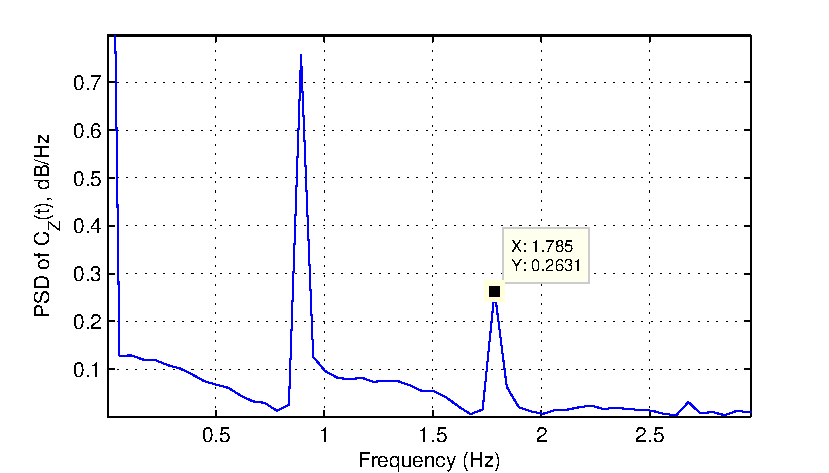
\includegraphics[width=100mm]{Cz_PSD_83_raw}
\caption{Power Spectrum Density map of $C_Z(t)$ of GTA in LAFO test with input $\alpha_0=30^o$, $\Delta \alpha = 25^o$ and $f=1 Hz$.}
\label{fig:GTA_Cz_psd}
\end{figure}

%The linear component of the model or the single-state VVM has successfully captured the frequency dependence of unsteady normal force variation due to small amplitude inputs. The identified model incorporates the dependence of in-phase and out-of-phase derivatives on the frequency of input in time-domain. Thus, it is useful for simulation of loads due to small amplitude change in angle-of-attack. For large amplitude change in angle-of-attack, variation of $C_Z(t)$ is nonlinear in nature.

The parameters $(a,K_1)$ as seen in Fig.(\ref{fig:GTA_Cz_Par}) are estimated only at $5^o$ intervals. This resolution is insufficient to realize the actual continuous model parameter functions. Hence, at this stage of estimation, the parameter functions $[a(\alpha),K_1(\alpha)]$ are defined by the estimated values of parameter bounds at the node-points and further refined using LAFO data. The resulting estimated parameter functions are indicated by red lines in Fig.(\ref{fig:GTA_Cz_Par}). It can be seen that this is different from the one defined by estimated values and their linear interpolation.
%\begin{figure}
% 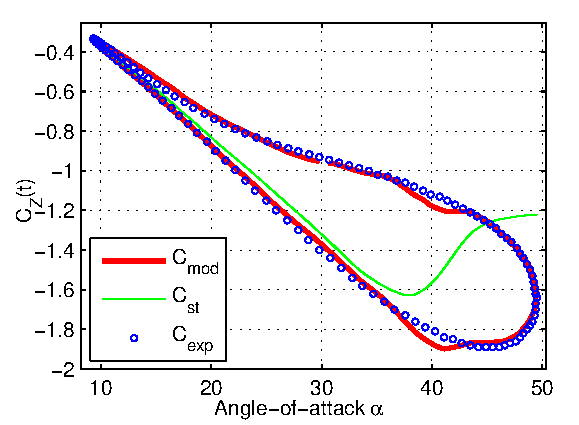
\includegraphics[width=74mm]{GTA_Cz_R63}
% \caption{Comparison of the output of VVM and wind tunnel test data, due to large amplitude oscillation input, for $C_Z$ of GTA,  $\alpha_0=30^o, \Delta \alpha =20^o, f=0.5 Hz$.}
%\label{fig:GTA_Cz_LA_sim}
%\end{figure}

The estimation of model parameters from LAFO data was performed using a specialized software called "Package for Interactive Identification" (PII), developed for this purpose by Goman and co-workers. The user manual of the software is in \cite{PIImanual1,PIImanual2}, and case studies on identification of nonlinear unsteady aerodynamic model using this software are given in \cite{GomanICAS94,GomanICAS97}. A combination of the gradient and steepest-descent algorithms is used in the optimization process. The software provides a Graphical-User-Interface to check the quality of fit-obtained and alter the options of the optimization process.

The estimated one-state VVM reproduces a qualitatively satisfactory output $C_Z(t)$ due to large amplitude change in angle-of-attack, but the accuracy is insufficient. The raw wind tunnel data from LAFO tests is examined to check the presence of harmonics. As seen in an example presented in Fig.(\ref{fig:GTA_Cz_psd}), PSD of $C_Z(t)$ has significant peaks at first and second harmonics of input frequency of $0.9 Hz$. This implies that a two-state VVM is sufficient for modeling $C_Z$. No such inference can be drawn for PDEM about the degree of polynomial term to be used in the model structure.

Now, the parameter functions $[a(\alpha),K_1(\alpha)]$ need to be tuned to capture the mild nonlinearities using LAFO data. From SAFO data, the parameter values of $[a(\alpha_0),K_1(\alpha_0)]$ are estimated only for $\alpha \in [35^o \, 55^o]$. The modeling and measurement noises in SAFO data are quantified by the error co-variance matrix, which in turn gives the bounds on $[a(\alpha_0), K_1(\alpha_0]$. As shown in Fig.(\ref{fig:GTA_Cz_Par}), the range of bounds is quite significant percentage of the mean value at most angle-of-attack. Hence, it is essential to tune $[a(\alpha),K_1(\alpha)]$ using the parameter bounds to account for the effects of noise as well as to estimate them over the extended range of $\alpha \in [25^o \, 60^o]$.
%
%
\begin{figure}
\centering
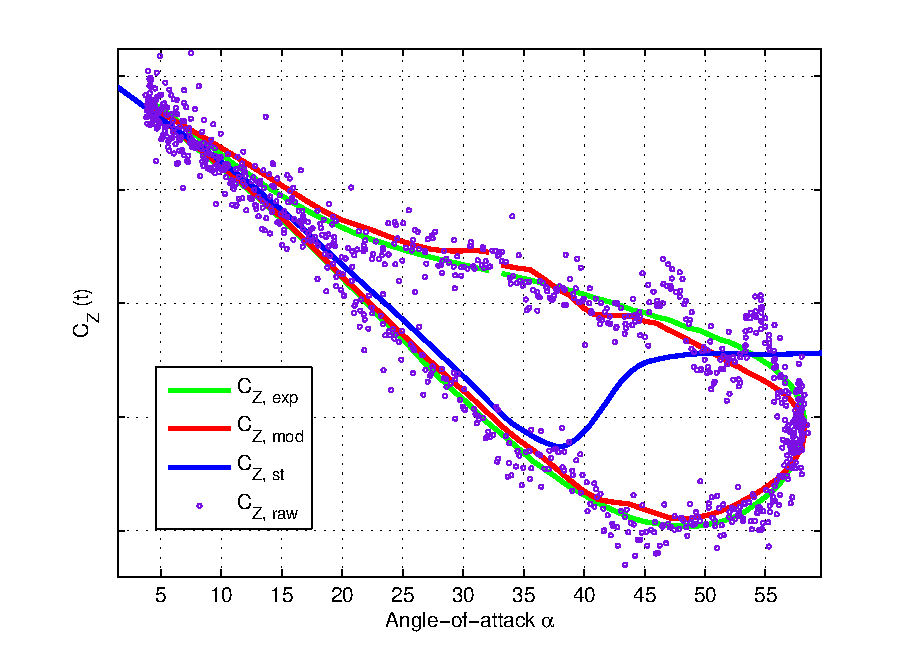
\includegraphics[width=100mm]{LA83_sim}
\caption{Comparison of VVM output with raw wind tunnel test data for $C_Z$ of GTA, due to sinusoidal input of $\alpha_0=30^o, \Delta \alpha =25^o, f=1 Hz$.}
\label{fig:GTA_Cz_R83}
\end{figure}

So, the functions $(a(\alpha), K_1(\alpha))$ are estimated considering these bounds as constraints and to produce a best fit with the LAFO data. The single-state VVM and Output-Error method are used in estimation of the parameter functions. An optimization is setup with root-mean-square-error between model output and experimental data as the cost function. Entire LAFO data is used simultaneously in the estimation process. It is found that the solution always converges to an approximately equivalent values of the parameter functions $a(\alpha)$ and $K_1(\alpha)$. These are indicated by red solid lines, overlaid on the estimated parameter bounds from SAFO data, in Fig.(\ref{fig:GTA_Cz_Par}). These estimated parameter functions are consistent with both SAFO and LAFO data.

The simulation results of the model thus obtained produce a good match with the LAFO data consistently. A sample of results of simulations is given in Fig.(\ref{fig:GTA_Cz_R83}). Only the steady state oscillation cycle generated by the model is plotted in the figure. In this figure, $C_{Z,raw}$ is the raw LAFo test data; $C_{Z,exp}$ is its reduction to steady oscillation cycle; $C_{Z,st}$ is the curve-fit of static test data and $C_{Z,mod}$ indicates the model output. The match between model output and experimental data shows minor inaccuracies.

This can be attributed to two issues. Firstly, the parameter function $K_1(\alpha)$ is especially nonlinear near $\alpha=40^o$, and estimation in this region is tricky. Secondly, the unsteady variation of load in this angle-of-attack region is very sensitive to external conditions like the vibration of sting. in parameter estimation only a steady state oscillation cycle which obtained by filtering the raw data over an appropriate bandwidth, and averaging the multiple oscillation cycles, is used. Hence, there is a need to examine raw wind tunnel test data to check the contribution of $x_2(t)$ is small in comparison to $x_1(t)$

In Fig.(\ref{fig:GTA_Cz_R83}) the model output is compared with the raw wind tunnel data. It is evident that the single-state VVM response is within the uncertainty limits of the raw wind tunnel data. This also shows that, if the second kernel state is included, it's value is in the error tolerance limits, and hence it may not be realistic. Hence a single-state VVM is of acceptable accuracy.



??? include the results and discussion using PDEM.

\subsection{Identification of Pitching moment coefficient of GTA}

Variations in $C_m(t)$ in the stall region are much more complex than that for the normal force coefficient. In some cases, $C_m(t)$ response to large amplitude sinusoidal input has three dynamic hysteresis loops which are associated with damping and anti-damping aerodynamic effects. Moreover, the mean value of these loops appears to be shifted from the steady state values obtained from static wind tunnel tests. Hence, the estimation problem is more challenging than the cases presented in literature like F16XL \cite{F16XLLong}, X31 \cite{X31}, Delta-$65^o$ \cite{AbramovThesis}, Delta-$70^o$ wings \cite{Nelson} and many other airfoils presented in literature \cite{Exp8Airfoil1}.
\begin{figure}[htbp]
\begin{center}
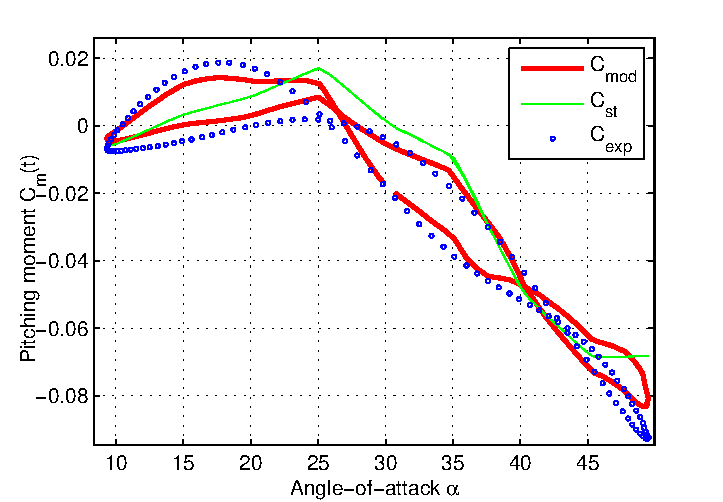
\includegraphics[width=100mm]{GTA_R63_Cm}
\caption{$C_m$ from VVM output and wind tunnel data.}
\label{fig:GTA_Cm_R63}
\end{center}
\end{figure}
\begin{figure}[htbp]
\begin{center}
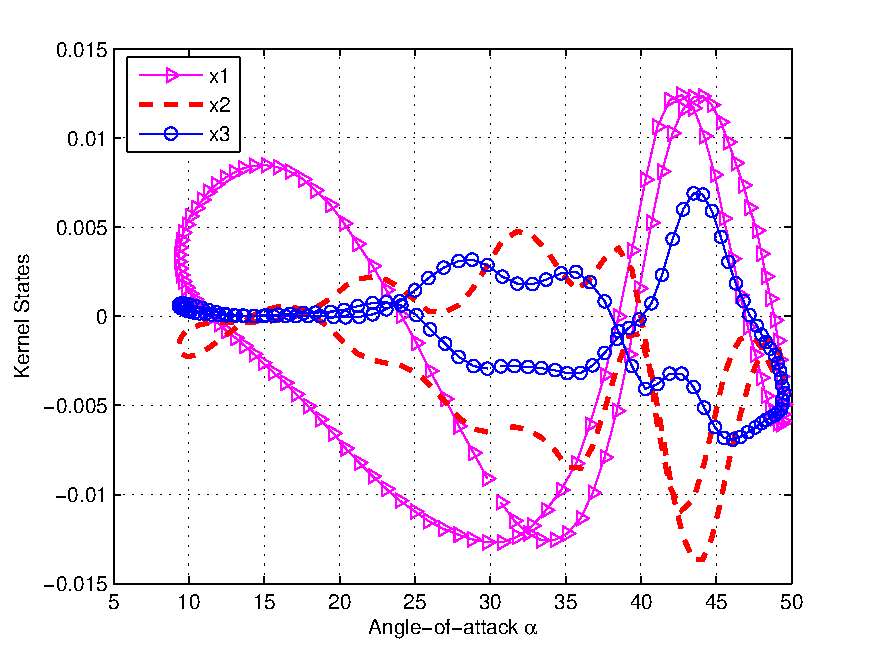
\includegraphics[width=100mm]{R63_kernelstates}
\caption{Kernel states of VVM.}
\label{fig:R63_kernelstates}
\end{center}
\end{figure}

Similar to the case of $C_Z(t)$, parameter estimation is performed by considering the bounds on $[a(\alpha_0),K_1(\alpha_0)]$ estimated from SAFO data as constraints, and estimating all the model parameter functions simultaneously. The node-points placed at $5^o$ intervals were found to be sufficient in the current estimation exercise.   The parameter function estimation procedure requires several iterations and adjustments in the number and location of node-points to get the best-fit, and it is an art at some level. The accuracy of the model is satisfactory for three-state VVM and consistent across all the LAFO data, as seen in the example in Fig.(\ref{fig:GTA_Cm_R63}).
%Fig.(\ref{fig:GTA_Cm_SA2}). 
 
 
Higher order kernel states $x_2(t)$ and $x_3(t)$ introduce significant nonlinear corrections, as evident from their relative magnitudes in Fig.(\ref{fig:R63_kernelstates}).  In the region of sharp stall $\alpha=[40^o \, 45^o]$, nonlinear corrections are particularly important. The second kernel produces a bias term in the harmonic input response of Volterra series, as proved in \cite{Bedrosian}. $x_2(t)$ is indeed seen to produce a bias component in $\alpha=[40^o \, 45^o]$ range, as expected from theory. Likewise, the third Volterra kernel produces significant correction in effective time-constant. In the current case study, $x_3(t)$ corrects damping and anti-damping oscillations in the angle-of-attack ranges $[30^o \, 35^o]$ and  $[40^o \, 45^o]$ respectively. This is also consistent with the analytical interpretations of Volterra kernel presented in \cite{OmranACC},and some of the applications to physiological systems presented in \cite{Marmerelis}. Therefore, kernel states $x_2(t)$ and $x_3(t)$ produce significant and systematic nonlinear corrections to the model response.

\begin{figure}[htbp]
\begin{center}
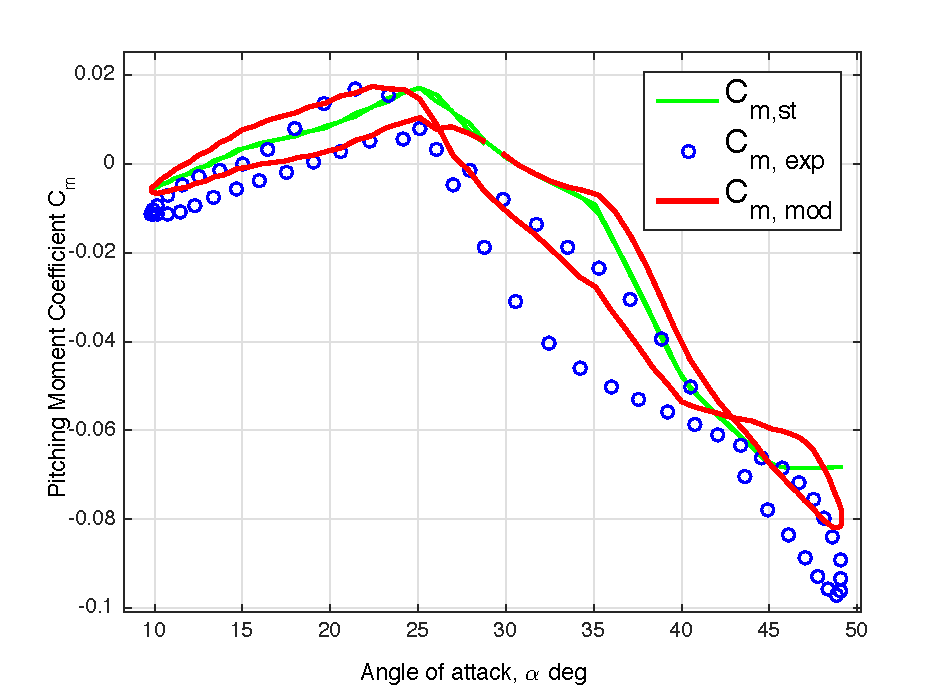
\includegraphics[width=100mm]{PDEM_Cm_R63}
\caption{$C_m$ from PDEM simulation output and wind tunnel data.}
\label{fig:PDEM_Cm_R63}
\end{center}
\end{figure}

Identification using PDEM has the estimation method using SAFO data as for VVM. The nonlinear model parameter functions $[K_{2}(\alpha), K_{3}(\alpha)]$ are estimated using LAFO data by output-error method and results are presented in Fig.(\ref{fig:PDEM_Cm_R63}). The results are satisfactory.


Typical variations in pitching moment coefficients of Delta-wing configurations are expected to be complex. This case study has amply illustrated the capability of a three state VVM to model complex dynamical nonlinearities in variation of unsteady aerodynamic loads, including shift of the cycle with respect to steady state value and multiple damping and anti-damping loops.


%\subsection{Identification of lateral-directional moment coefficients Delta-$65^o$ Wing}
%\begin{enumerate}
%\item Linear relation between in-phase and out-of-phase derivatives of Cl, Cn
%\item Estimated parameters from SAFO data, with bounds of Cl, Cn
%\item Power spectrum density of LAFO for Cl and Cn
%\item Simulation results for VVM1, VVM3 and PDEM3 of Cm
%\end{enumerate}

\subsection{Comparative analysis of VVM and PoDE}
Comparison of accuracy in terms of RMS error in multiple cases. Explanation of different effects caused by nonlinear term parameters on time-scale parameters. Single stable solution constraint on PDEM. Use in presence of static hysteresis.

\section{Influence on Flight Dynamics}
In this section, affect of unsteady loads on aircraft dynamic modes is presented using a simple frequency domain spectrum analysis. The industry-grade aero-databases are in the form of a large set of multi-dimensional data-tables and an application rule. The VVM and PDEM models are integrated with the available aero-database, as these are formulated as an incremental contribution of unsteady aerodynamic loads.

For the purpose of simulation, the differential equations of VVM or PDEM are augmented to the 6DOF rigid-body equations of motion of the aircraft, and the parameter functions are included as tables in the aero-database. Therefore, the aircraft flight dynamics now has two additional states. Thus, these models can be seamlessly and simply be used in 6DOF simulation studies.

The fast flight dynamic modes are of primary interest in this analysis. This is because the dynamics of slower modes is effected by unsteady aerodynamics to a much lesser extent and it can be corrected by the pilot or the autopilot control laws. Hence, in flight dynamic analysis using a $5^{th}$ order set of the states $(\alpha, \beta, p, q, r)$ is sufficient, as discussed in \cite{GomanAES1,GomanAES2}. This set corresponds to flight dynamic modes of Short-period, Roll-subsidence and Dutch-roll. The time-scales of these modes are one order of magnitude smaller than the slower modes like Phugoid and Spiral. Hence, the analysis using this reduced set of equations of motion is unaffected by the slower modes.

The $5^{th}$-order setup is subject to trim, linearization and stability analysis. An altitude of $H=6000 m$ and Mach number $M=0.4$ are used in this analysis. At trim points, $\dot{\alpha}=0$ and hence the steady-state solutions of Eq.(\ref{eq:VVMfun1}) are $[C_{Z_d},C_{m_d}]=[0,0]$. So, the trim solutions are obtained at the same aircraft kinematic states $(\alpha, \beta, p, q, r)$ as that from an aero-database without unsteady model. Therefore, the unsteady model does not effect the trim solutions directly, but causes difference in the transient dynamics between two steady states. The longitudinal trim solutions were investigated in the range $\alpha \in [28^o \, 40^o]$, and there were no trim solutions beyond this angle-of-attack.
%
%\begin{figure}
% \begin{subfigmatrix}{1}% number of columns
%  \subfigure{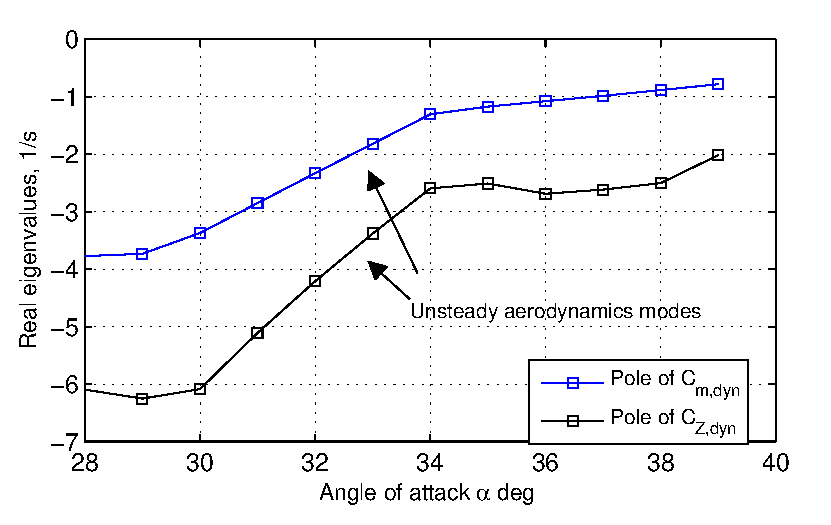
\includegraphics[scale=0.9]{Rlocus_alpha}}
%  \subfigure{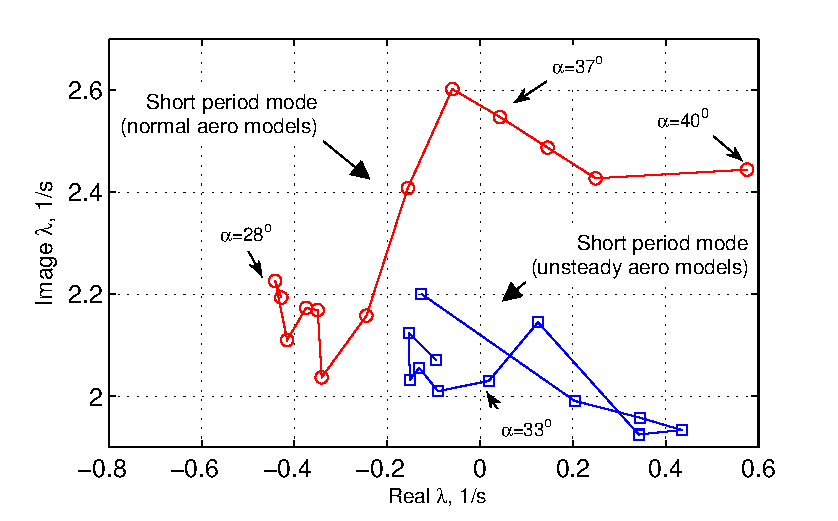
\includegraphics[scale=0.9]{Rlocus_SP}}
% \end{subfigmatrix}
% \caption{Eigenvalue analysis to characterize the effect of longitudinal unsteady aerodynamics on longitudinal modes, at altitude $6000 m$ and Mach $0.4$}
% \label{fig:FMUnst}
%\end{figure}



\begin{figure}[tb]
\begin{center}
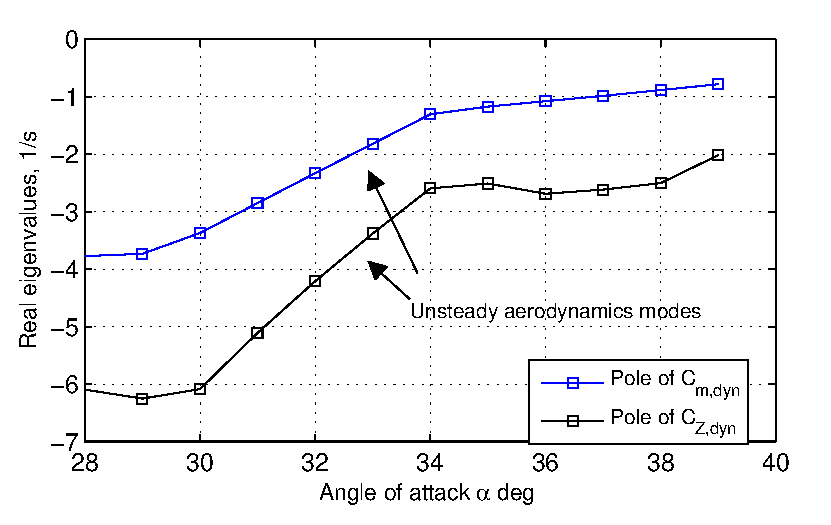
\includegraphics[width=100mm]{Rlocus_alpha}
\caption{Real-part of the eigenvalues of unsteady components of $C_a$ and $C_m$}
\label{fig:Rlocus_alpha}
\end{center}
\end{figure}
\begin{figure}[tb]
\begin{center}
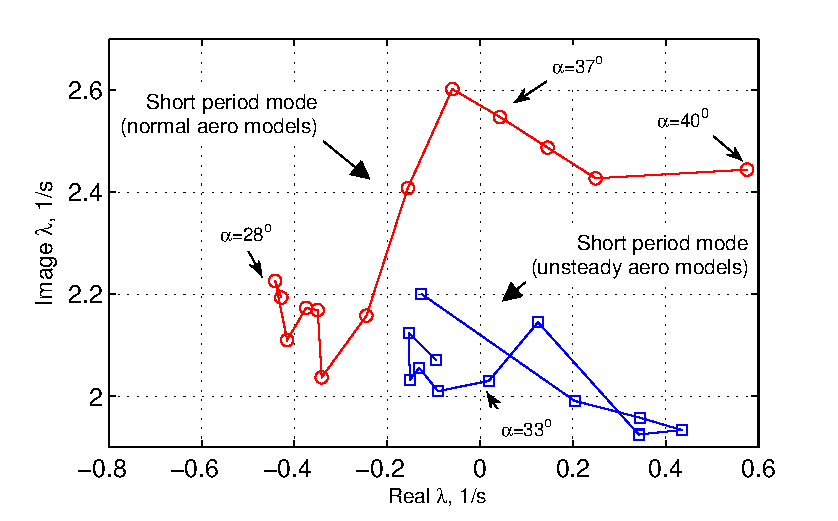
\includegraphics[width=100mm]{Rlocus_SP}
\caption{Root-locus of positive eigenvalue of Short-Period mode}
\label{fig:Rlocus_SP}
\end{center}
\end{figure}

The unsteady models are found to effect the stability properties of the trim solutions. Since the linear stability analysis is valid for a small range of angle-of-attack around the trim-point, only the first kernel state of VVM is used in this analysis. The dynamics equations are linearized at trim points, and their eigen-spectrum shows the affect on modes. The unsteady model states $C_{Z_d}(t),C_{m_d}(t)$ create two additional poles (eigenvalues). 

A locus of the two real eigenvalues produced by the unsteady model states for $\alpha \in [28^o \, 40^o]$ is presented in Fig.(\ref{fig:Rlocus_alpha}). The real-part of the poles move closer tp zero with increasing angle-of-attack. Thus, the effect of unsteady modes becomes important as the aircraft enters stall angle-of-attack region; and their effect on flight dynamics becomes more prominent. These poles repel the eigenvalues of other modes away from them, and hence affect other flight modes significantly.

Now consider the root-locus of the positive frequency of the short-period complex conjugate pair of eigenvalues. The first root-locus is obtained using the aero-database with the values of aero-derivative for frequency $f= 1 Hz$ from SAFO data. The second root-locus is for VVM, which accommodates the frequency dependence of damping derivatives in the form of unsteady model poles. A comparison of these two root-locii is presented in Fig.(\ref{fig:Rlocus_SP}). While the first root-locus shows that the Short-period pole crosses imaginary axis and becomes unstable at $\alpha > 36^o$; the second root-locus shows that this happens at $\alpha > 32^o$. There is also significant difference in the Short-period mode frequency for the entire angle-of-attack range. These two results show that there can be a significant error in control-law design if the unsteady aerodynamic effects are not properly included in the model.

In the control-law design, the effect of unmodeled dynamics is expected to be accommodated by the robustness of estimated feedback control loop-gains. However, even in this case the handling qualities of the closed-loop aircraft dynamics are likely to be severely effected as shown in \cite{Abramov2}.

The role of nonlinearity in unsteady variation of aerodynamic loads is not evident from linear stability analysis. The nonlinear stability of the trim points in the stall angle-of-attack regimes is characterized by the Region-of-attraction of a trim solution. It is usually bounded and defines the level of critical disturbances. GTA was found to have unstable equilibrium states for lateral-directional modes in the stall angle-of-attack regimes. Close to the boundary of this unstable region, the stable equilibriums have limited stability region. An accurate model of nonlinear unsteady aerodynamics is important for correct prediction of critical external disturbances for stability of a flight mode.

\section{Conclusions}



%\section{Conclusion}
%Although a conclusion may review the main points of the paper, it must not replicate the abstract. A conclusion might elaborate on the importance of the work or suggest applications and extensions. Do not cite references in the conclusion. Note that the conclusion section is the last section of the paper to be numbered. The appendix (if present), acknowledgment, and references are listed without numbers.
%
%\section*{Appendix}
%
%An Appendix, if needed, appears before the acknowledgments.

\section*{Acknowledgments}
Authors acknowledge the partial financial support from ADA,Bangalore for doing this work.

\section*{References}

\bibliographystyle{aiaa}
\bibliography{ThesisRef}

\end{document}
